% Options for packages loaded elsewhere
\PassOptionsToPackage{unicode}{hyperref}
\PassOptionsToPackage{hyphens}{url}
%
\documentclass[
]{book}
\usepackage{amsmath,amssymb}
\usepackage{iftex}
\ifPDFTeX
  \usepackage[T1]{fontenc}
  \usepackage[utf8]{inputenc}
  \usepackage{textcomp} % provide euro and other symbols
\else % if luatex or xetex
  \usepackage{unicode-math} % this also loads fontspec
  \defaultfontfeatures{Scale=MatchLowercase}
  \defaultfontfeatures[\rmfamily]{Ligatures=TeX,Scale=1}
\fi
\usepackage{lmodern}
\ifPDFTeX\else
  % xetex/luatex font selection
\fi
% Use upquote if available, for straight quotes in verbatim environments
\IfFileExists{upquote.sty}{\usepackage{upquote}}{}
\IfFileExists{microtype.sty}{% use microtype if available
  \usepackage[]{microtype}
  \UseMicrotypeSet[protrusion]{basicmath} % disable protrusion for tt fonts
}{}
\makeatletter
\@ifundefined{KOMAClassName}{% if non-KOMA class
  \IfFileExists{parskip.sty}{%
    \usepackage{parskip}
  }{% else
    \setlength{\parindent}{0pt}
    \setlength{\parskip}{6pt plus 2pt minus 1pt}}
}{% if KOMA class
  \KOMAoptions{parskip=half}}
\makeatother
\usepackage{xcolor}
\usepackage{longtable,booktabs,array}
\usepackage{calc} % for calculating minipage widths
% Correct order of tables after \paragraph or \subparagraph
\usepackage{etoolbox}
\makeatletter
\patchcmd\longtable{\par}{\if@noskipsec\mbox{}\fi\par}{}{}
\makeatother
% Allow footnotes in longtable head/foot
\IfFileExists{footnotehyper.sty}{\usepackage{footnotehyper}}{\usepackage{footnote}}
\makesavenoteenv{longtable}
\usepackage{graphicx}
\makeatletter
\def\maxwidth{\ifdim\Gin@nat@width>\linewidth\linewidth\else\Gin@nat@width\fi}
\def\maxheight{\ifdim\Gin@nat@height>\textheight\textheight\else\Gin@nat@height\fi}
\makeatother
% Scale images if necessary, so that they will not overflow the page
% margins by default, and it is still possible to overwrite the defaults
% using explicit options in \includegraphics[width, height, ...]{}
\setkeys{Gin}{width=\maxwidth,height=\maxheight,keepaspectratio}
% Set default figure placement to htbp
\makeatletter
\def\fps@figure{htbp}
\makeatother
\setlength{\emergencystretch}{3em} % prevent overfull lines
\providecommand{\tightlist}{%
  \setlength{\itemsep}{0pt}\setlength{\parskip}{0pt}}
\setcounter{secnumdepth}{5}
\usepackage{booktabs}
\usepackage{amsthm}
\makeatletter
\def\thm@space@setup{%
  \thm@preskip=8pt plus 2pt minus 4pt
  \thm@postskip=\thm@preskip
}
\makeatother
\ifLuaTeX
  \usepackage{selnolig}  % disable illegal ligatures
\fi
\usepackage[]{natbib}
\bibliographystyle{apalike}
\IfFileExists{bookmark.sty}{\usepackage{bookmark}}{\usepackage{hyperref}}
\IfFileExists{xurl.sty}{\usepackage{xurl}}{} % add URL line breaks if available
\urlstyle{same}
\hypersetup{
  pdftitle={G8 Biology Guidebook},
  pdfauthor={Page Tsien},
  hidelinks,
  pdfcreator={LaTeX via pandoc}}

\title{G8 Biology Guidebook}
\author{\href{https://pagius5.github.io/}{Page Tsien}}
\date{2024-10-21}

\begin{document}
\maketitle

{
\setcounter{tocdepth}{1}
\tableofcontents
}
\hypertarget{overview}{%
\chapter{Overview}\label{overview}}

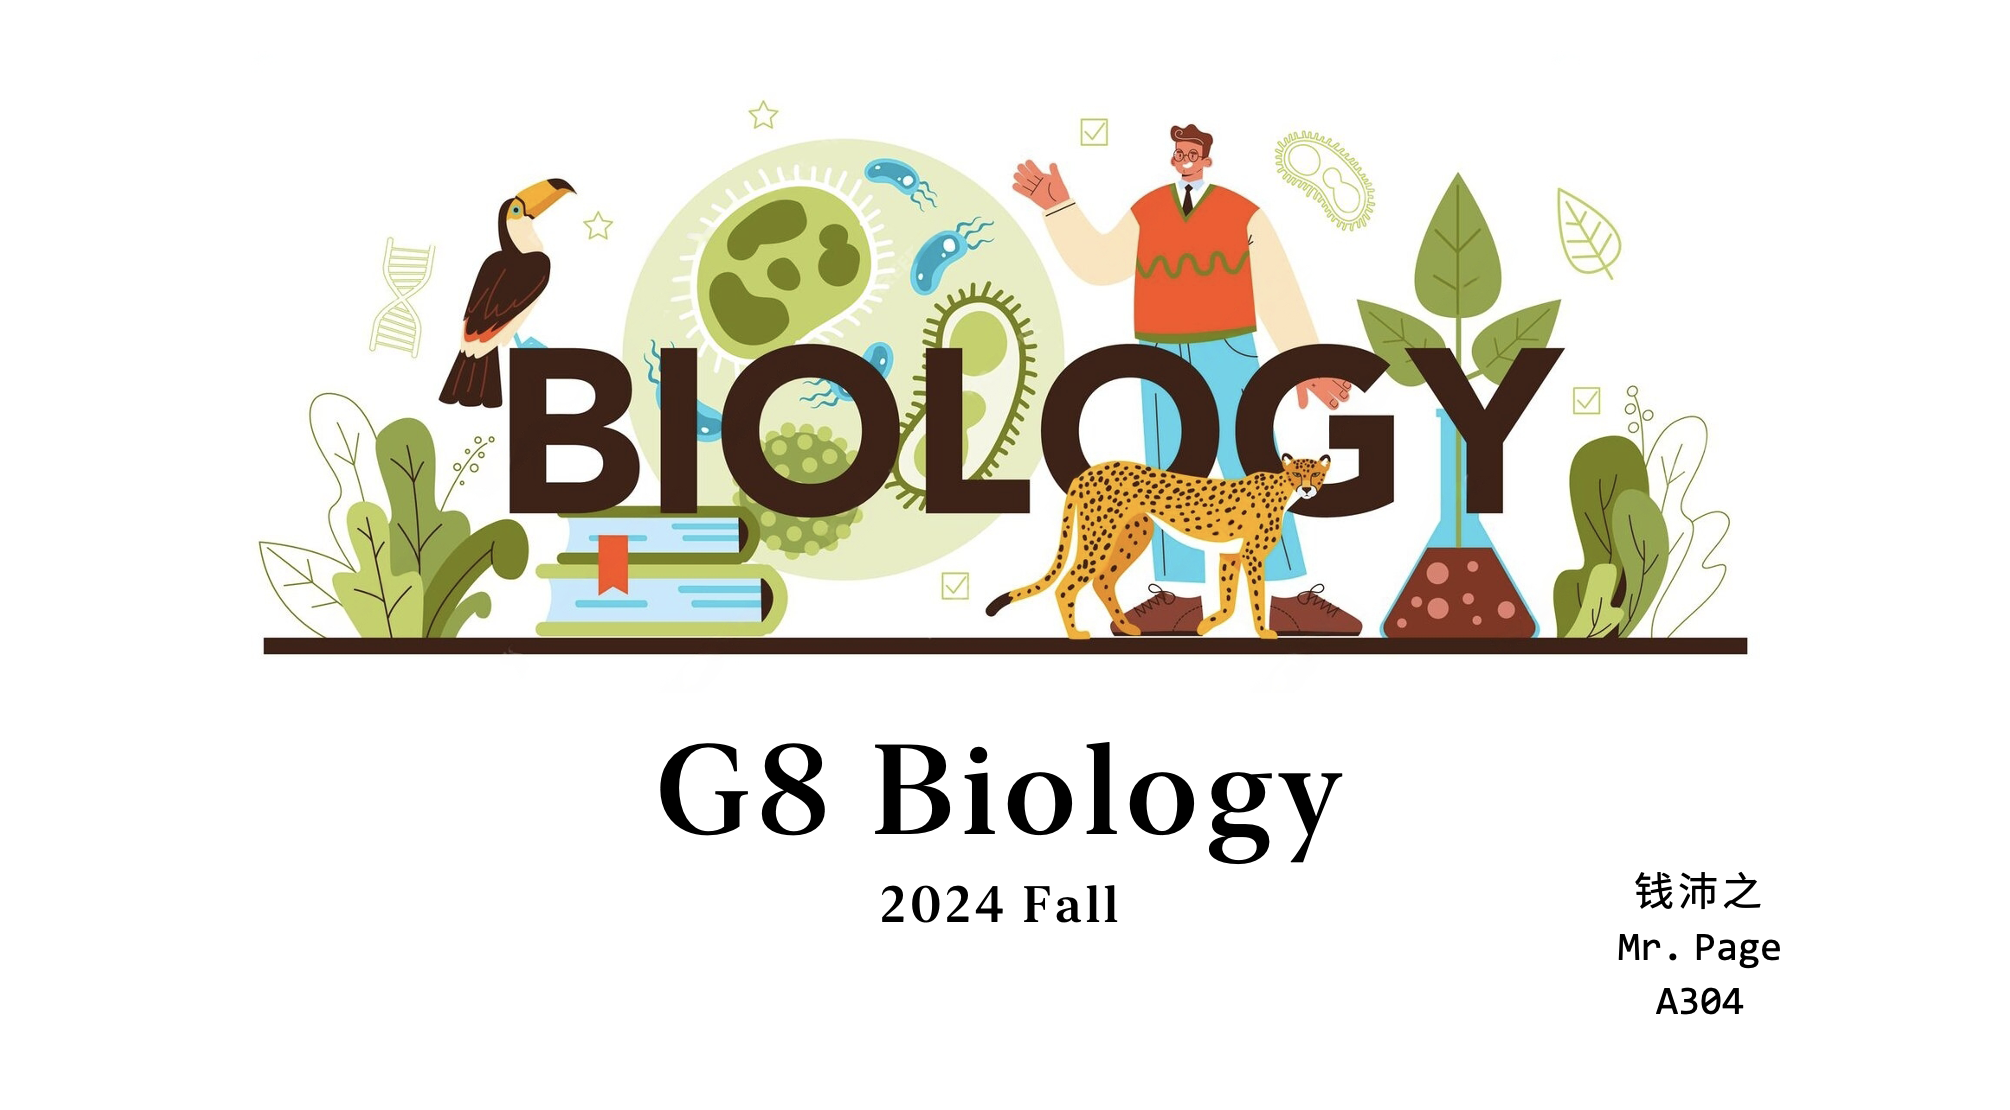
\includegraphics{./img/g8-bio.png}

\hypertarget{chapter-i-from-a-cell-to-an-organism}{%
\chapter{Chapter I: From A Cell To An Organism}\label{chapter-i-from-a-cell-to-an-organism}}

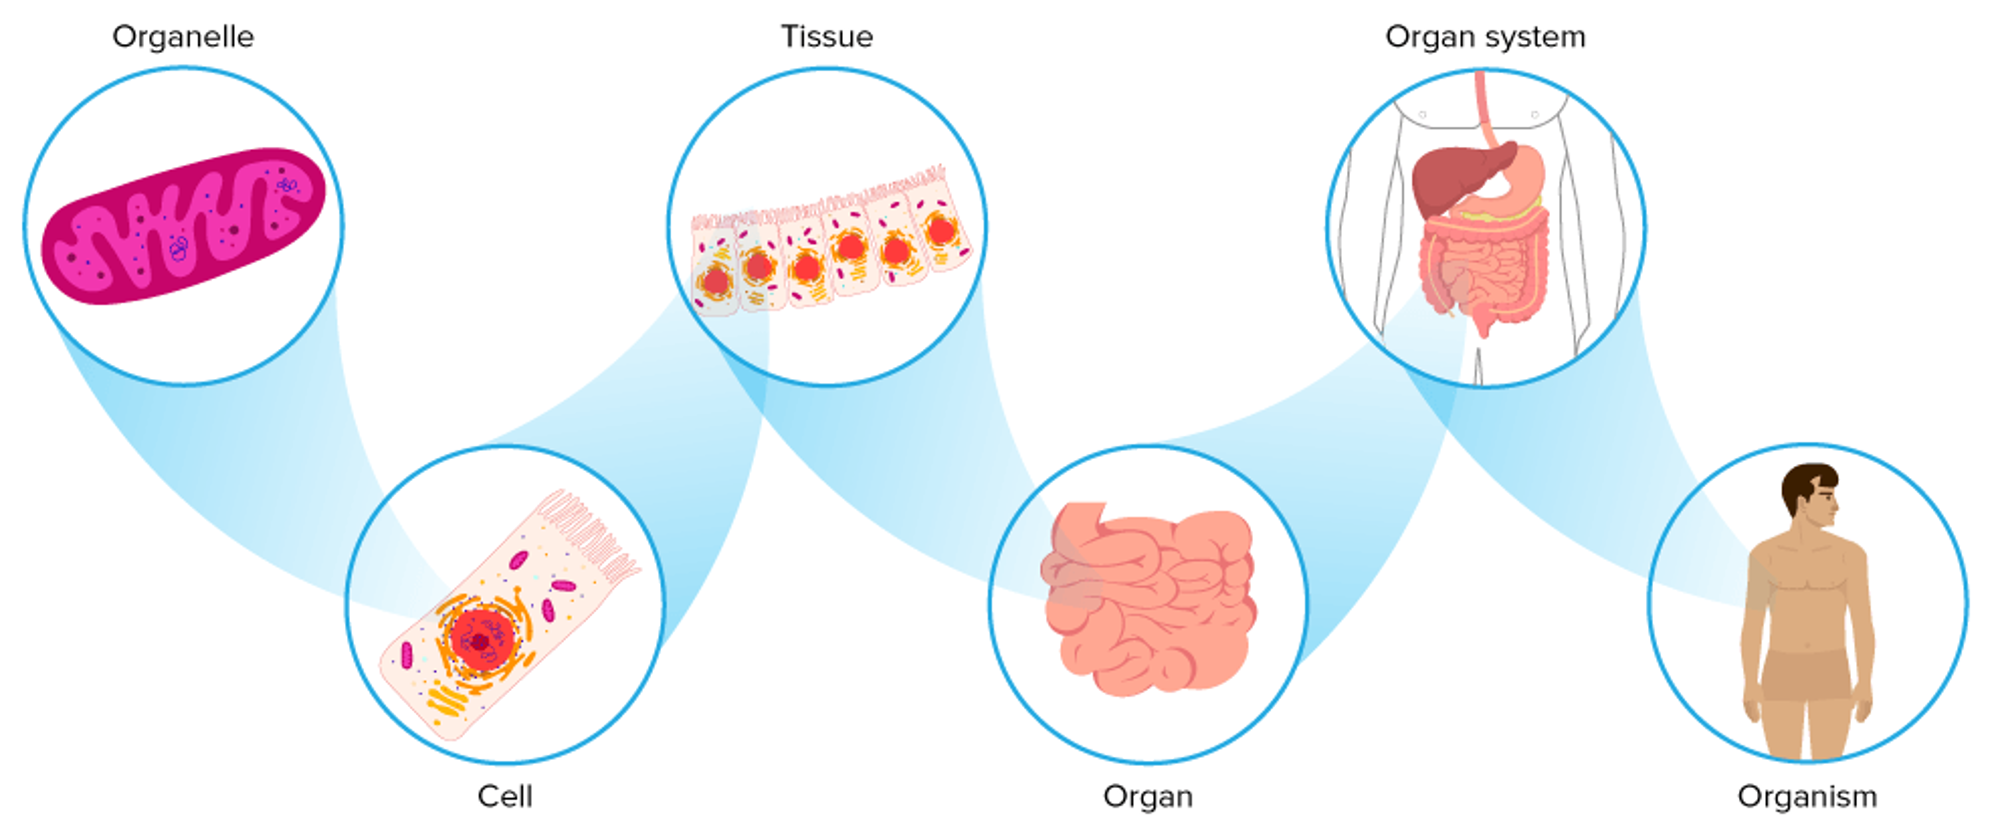
\includegraphics{./img/ch1.png}

\hypertarget{lecture-1-cell-cycle}{%
\section{Lecture 1: Cell Cycle}\label{lecture-1-cell-cycle}}

\hypertarget{lecture-2-cell-division}{%
\section{Lecture 2: Cell Division}\label{lecture-2-cell-division}}

\hypertarget{lecture-3-levels-of-organization}{%
\section{Lecture 3: Levels of Organization}\label{lecture-3-levels-of-organization}}

\hypertarget{experiment-1-observing-mitosis-in-plant-cells}{%
\section{Experiment 1: Observing Mitosis In Plant Cells}\label{experiment-1-observing-mitosis-in-plant-cells}}

\hypertarget{experiment-2-cell-differentiation}{%
\section{Experiment 2: Cell Differentiation}\label{experiment-2-cell-differentiation}}

\hypertarget{project-1-mitosis-the-cell-cycle}{%
\section{Project 1: Mitosis \& The Cell Cycle}\label{project-1-mitosis-the-cell-cycle}}

\hypertarget{project-2-biological-organization}{%
\section{Project 2: Biological Organization}\label{project-2-biological-organization}}

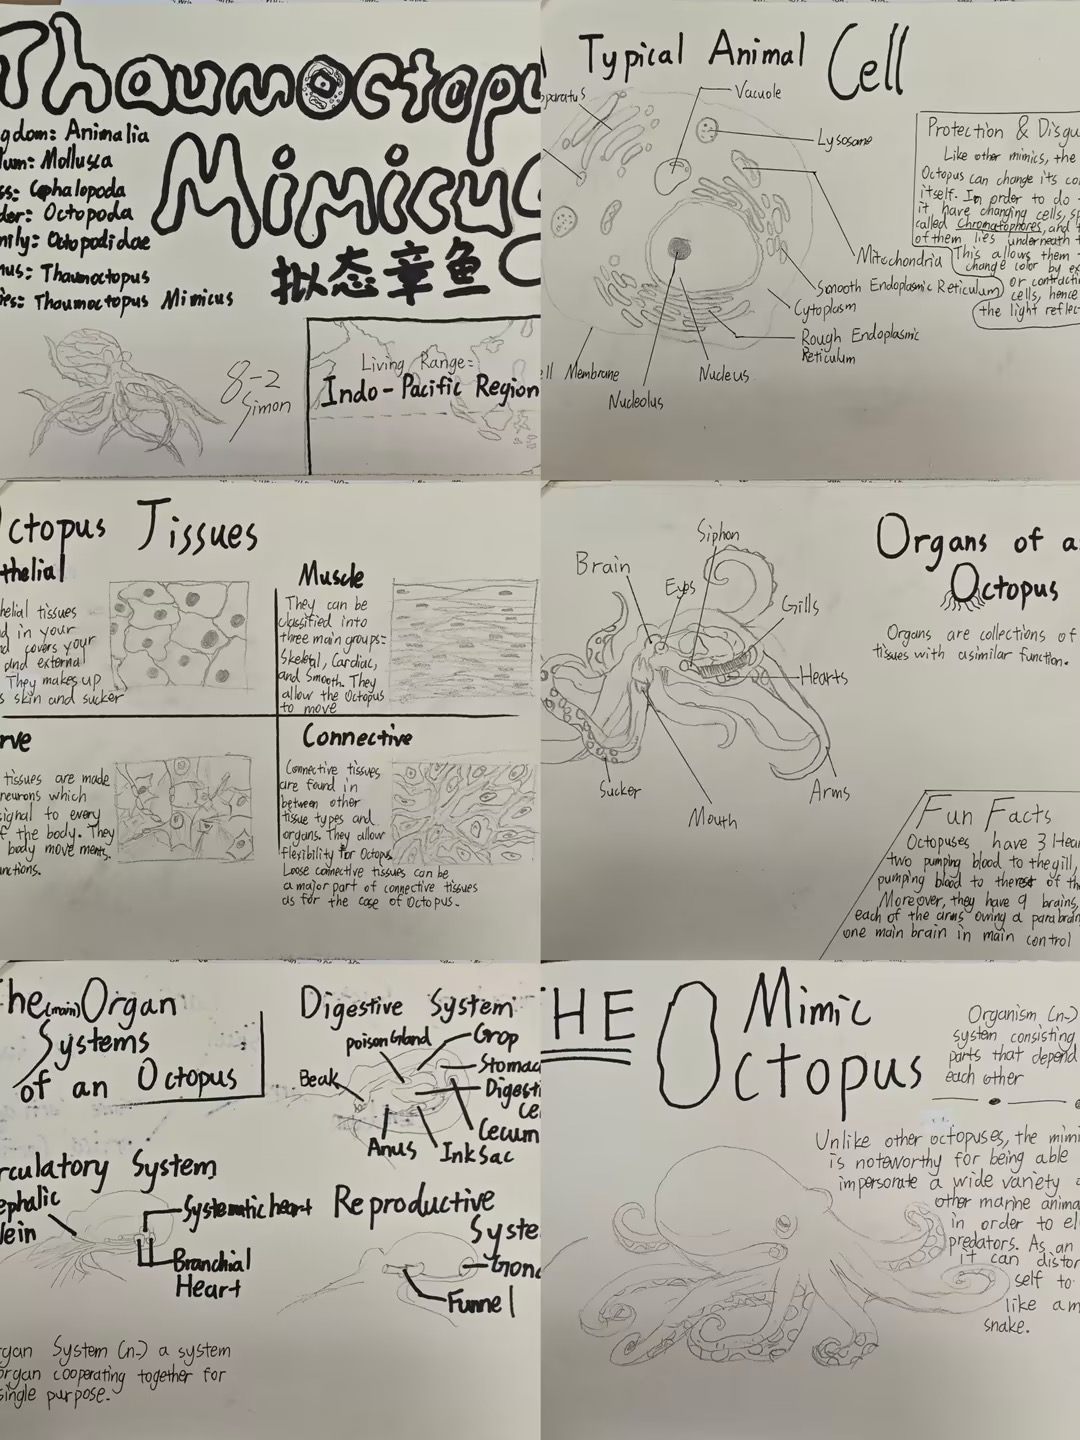
\includegraphics{./img/p2-1.jpg}

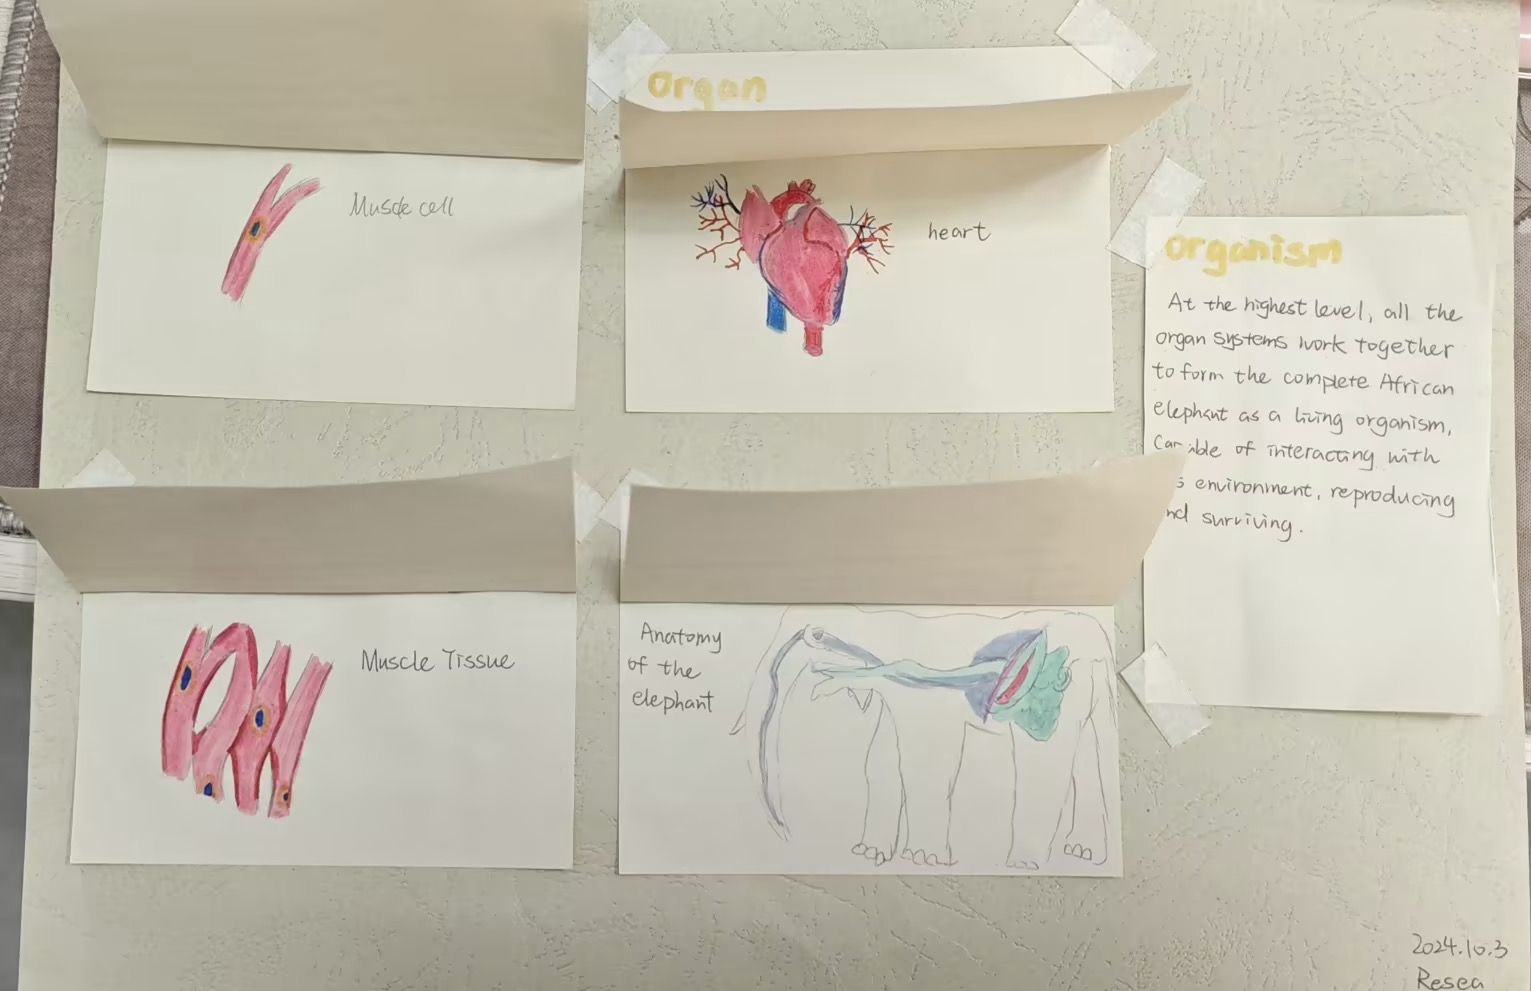
\includegraphics{./img/p2-2.jpg}

\hypertarget{chapter-ii-reproduction-of-organisms}{%
\chapter{Chapter II: Reproduction Of Organisms}\label{chapter-ii-reproduction-of-organisms}}

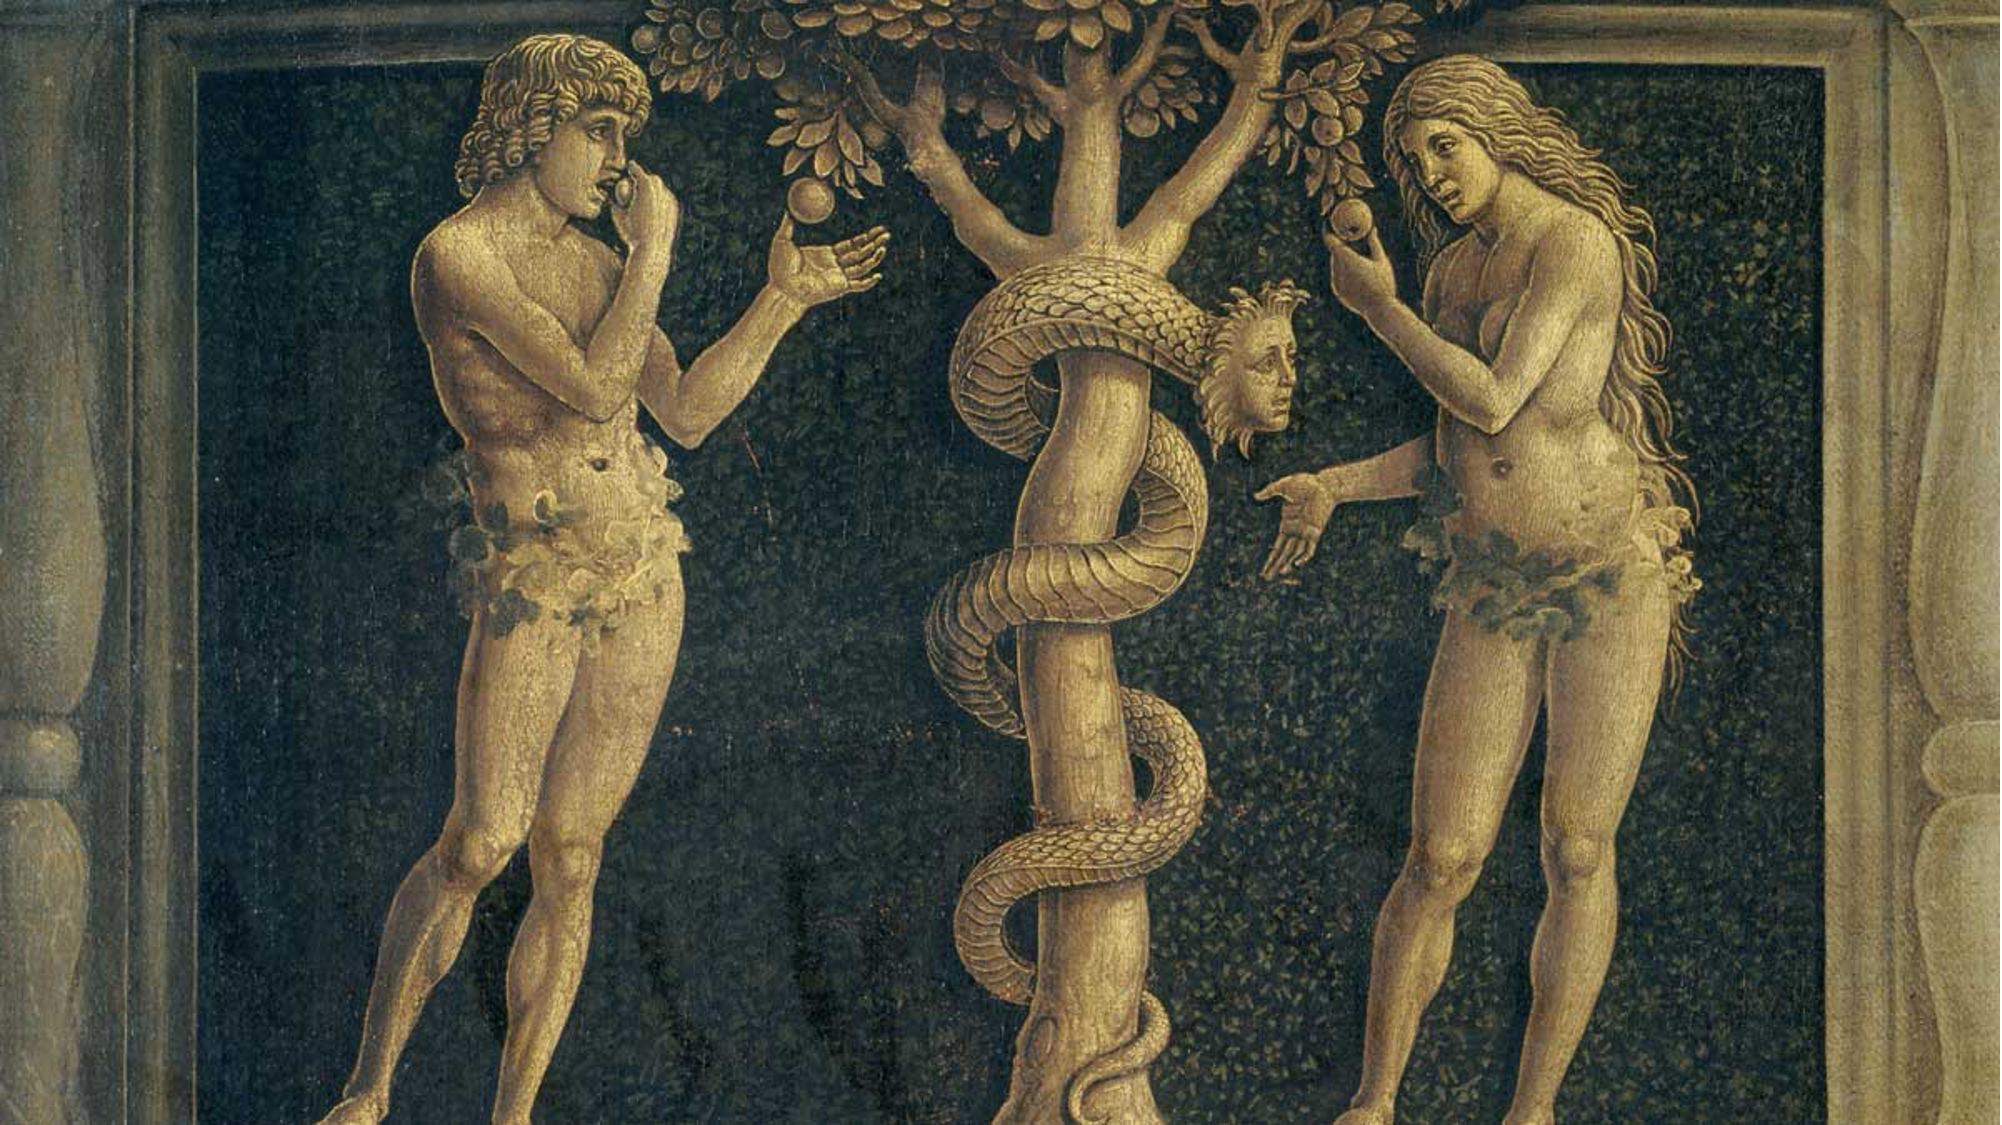
\includegraphics{./img/ch2.png}

\hypertarget{lecture-4-sexual-reproduction}{%
\section{Lecture 4: Sexual Reproduction}\label{lecture-4-sexual-reproduction}}

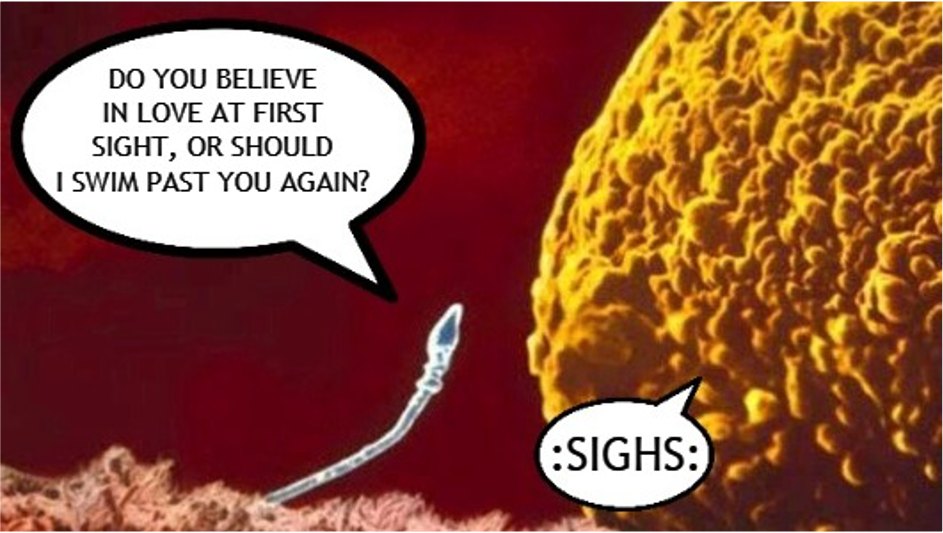
\includegraphics{./img/sperm-egg-meme.png}

\hypertarget{keywords}{%
\subsection{Keywords}\label{keywords}}

\begin{longtable}[]{@{}cc@{}}
\toprule\noalign{}
英文 & 中文 \\
\midrule\noalign{}
\endhead
\bottomrule\noalign{}
\endlastfoot
Sexual Reproduction & 有性生殖 \\
Meiosis & 减数分裂 \\
Sperm & 精子 \\
Egg & 卵子 \\
Fertilization & 受精 \\
Zygote & 受精卵 \\
Haploid & 单倍体 \\
Diploid & 二倍体 \\
Homologous chromosomes & 同源染色体 \\
\end{longtable}

\hypertarget{lesson-outline}{%
\subsection{Lesson outline}\label{lesson-outline}}

\textbf{A. What is sexual reproduction?}\\
1. {Sexual reproduction} produces an offspring when genetic materials from two
different sex cells combine.\\
a. The female sex cell, a(n) {egg}, forms in an ovary.\\
b. The male sex cell, a(n) {sperm}, forms in a testis.\\
2. During a process called {fertilization}, an egg cell and a sperm cell join together. The
new cell that forms is called a(n) {zygote}.

\textbf{B. Diploid Cells}\\
1. Organisms that reproduce sexually make two kinds of cells---{body} cells and sex cells.\\
2. Body cells are {diploid}; they have pairs of chromosomes.\\
3. If a zygote has too many or too few {chromosomes}, it will not develop properly.\\
4. Different organisms have different {numbers} of chromosomes.\\
5. {Homologous chromosomes} are pairs of chromosomes that have genes for the same traits arranged in the same order.

\textbf{C. Haploid Cells}\\
1. Sex cells are {haploid}; they have only one chromosome from each pair of chromosomes.\\
2. In {meiosis}, one diploid cell divides and makes four haploid cells.

\hypertarget{homework}{%
\subsection{Homework}\label{homework}}

\textbf{Matching}\\
1. G\\
2. B\\
3. H\\
4. C\\
5. I\\
6. A\\
7. D\\
8. F\\
9. E

\textbf{Multiple Choice Questions}\\
10. A\\
11. B

\textbf{Short Answer Questions}\\
12. Sexual reproduction is the {production of an offspring} that results when the genetic material from two different cells combine.\\
(Hint: Check ``how to write a definition'' in extension)\\
{s}\\
13. A zygote is {a new cell} that forms when an egg cell and a sperm cell join during fertilization.\\
(Hint: Check ``how to write a definition'' in extension)\\
{s}\\
14. A diploid cell has {pairs of chromosomes} and is located in body cells. A haploid cell has only {one set of chromosomes} and is located in sex cells.\\
(Hint: a pair or chromosomes/two sets of chromosomes vs.~one chromosome from each pair/one set of chromsomes)

\hypertarget{extension}{%
\subsection{Extension}\label{extension}}

\textbf{How to write a definition?}

A formal definition is based upon a concise, logical pattern that includes as much information as it can within a minimum amount of space. The primary reason to include definitions in your writing is to avoid misunderstanding with your audience. A formal definition consists of three parts:

\begin{enumerate}
\def\labelenumi{\arabic{enumi}.}
\tightlist
\item
  The \textbf{term} (word or phrase) to be defined\\
\item
  The \textbf{class} of object or concept to which the term belongs\\
\item
  The \textbf{differentiating characteristics} that distinguish it from all others of its class
\end{enumerate}

For example:

\begin{itemize}
\tightlist
\item
  Water (term) is a liquid (class) made up of molecules of hydrogen and oxygen in the ratio of 2 to 1 (differentiating characteristics).\\
\item
  Comic books (term) are sequential and narrative publications (class) consisting of illustrations, captions, dialogue balloons, and often focus on super-powered heroes (differentiating characteristics).\\
\item
  Astronomy (term) is a branch of scientific study (class) primarily concerned with celestial objects inside and outside of the earth's atmosphere (differentiating characteristics).
\end{itemize}

Sources:\\
1. \url{https://owl.purdue.edu/owl/general_writing/common_writing_assignments/definitions.html}\\
2. \url{https://www.sjsu.edu/aanapisi/docs/DefinitonLessonPlanbyEdSams.pdf}

\hypertarget{lecture-5-meiosis-1}{%
\section{Lecture 5: Meiosis-1}\label{lecture-5-meiosis-1}}

\hypertarget{lesson-outline-1}{%
\subsection{Lesson outline}\label{lesson-outline-1}}

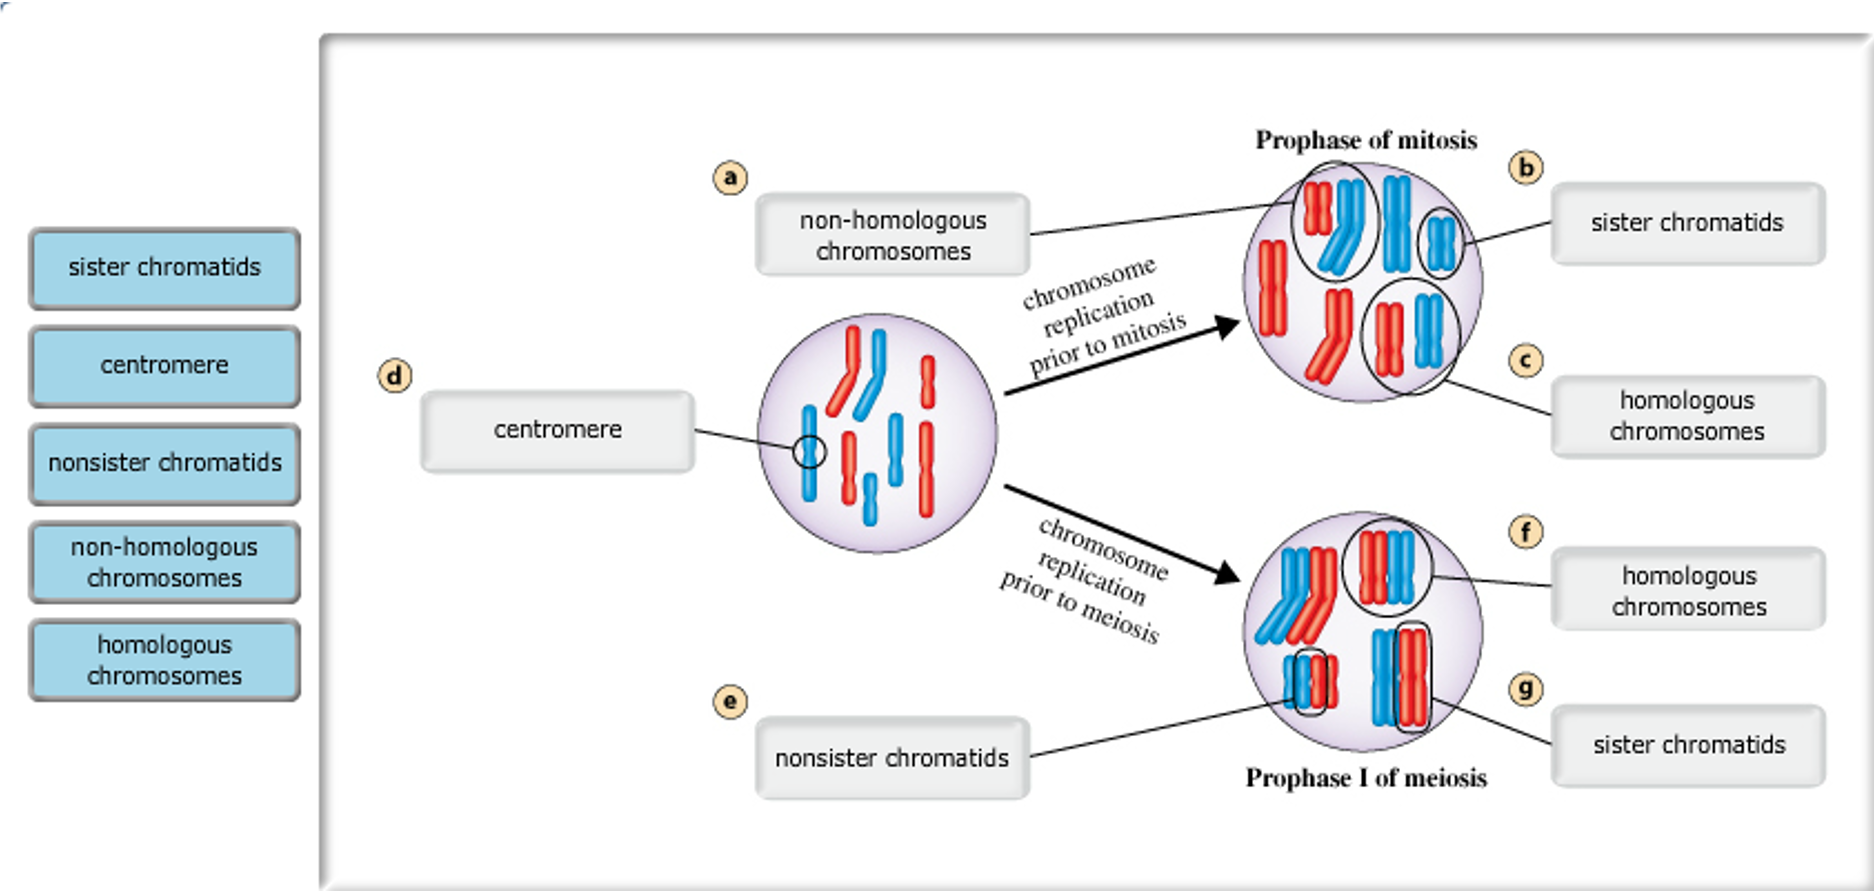
\includegraphics{./img/nonsis.png}

\textbf{D. The Phases of Meiosis}\\
1. Meiosis involves two divisions of the nucleus and the {cytoplasm}. These divisions, known as meiosis I and meiosis II, result in four haploid cells.\\
2. During {interphase}, the reproductive cell grows and duplicates its chromosomes.\\
3. During meiosis I, each pair of duplicated homologous chromosomes {separates}.\\
4. After meiosis I, the two cells formed during this stage go through a second division of the {nucleus} and cytoplasm called meiosis II. During meiosis II, sister {chromatids} separate to produce four haploid cells.

\textbf{E. Why is meiosis important?}\\
1. Meiosis forms sex cells with the correct haploid number of {chromosomes}. This maintains the correct {diploid} number of chromosomes in organisms when sex cells join. Meiosis creates genetic variation by producing {haploid} cells.

\hypertarget{homework-1}{%
\subsection{Homework}\label{homework-1}}

\textbf{Fill in the Blanks}\\
1. diploid; haploid\\
2. haploid; diploid\\
3. diploid\\
4. homologous chromosomes\\
5. homologous chromosomes\\
6. N/A\\
7. meiosis\\
8. sister chromatids\\
9. sister chromatids\\
10. meiosis; meiosis\\
11. meiosis

\textbf{Short Answer Questions}\\
12. Sex cells are haploid cells.

\hypertarget{lecture-6-meiosis-2}{%
\section{Lecture 6: Meiosis-2}\label{lecture-6-meiosis-2}}

\hypertarget{lesson-outline-2}{%
\subsection{Lesson outline}\label{lesson-outline-2}}

\begin{longtable}[]{@{}c@{}}
\toprule\noalign{}
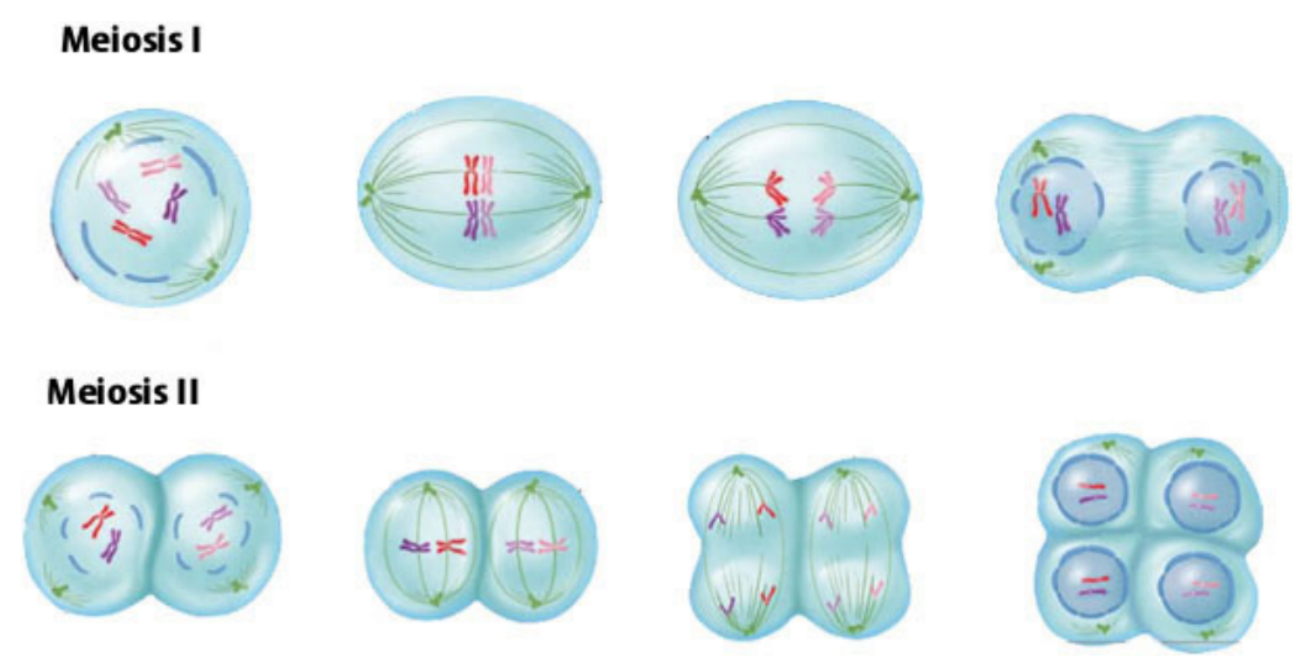
\includegraphics{./img/meiosis2.png} \\
\midrule\noalign{}
\endhead
\bottomrule\noalign{}
\endlastfoot
\emph{meiosis illustration 1} \\
\end{longtable}

\begin{longtable}[]{@{}c@{}}
\toprule\noalign{}
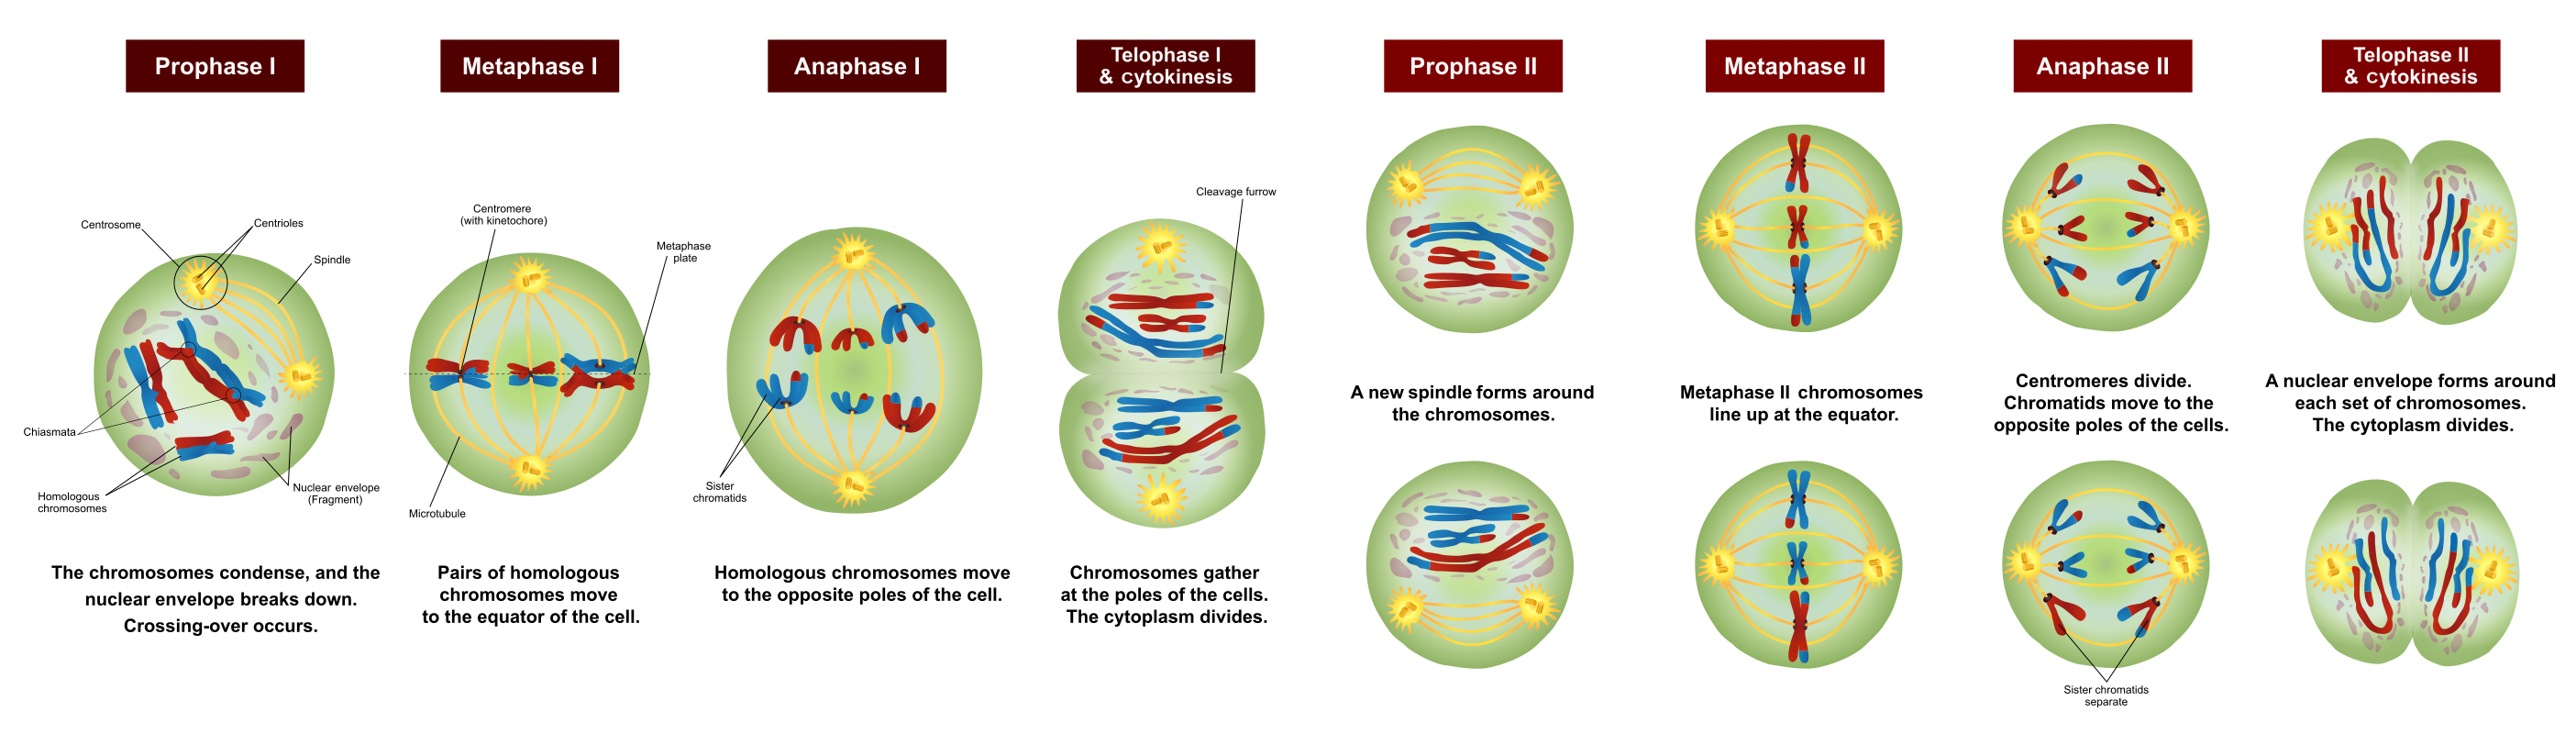
\includegraphics{./img/Meiosis_Stages.svg.png} \\
\midrule\noalign{}
\endhead
\bottomrule\noalign{}
\endlastfoot
\emph{meiosis illustration 2} \\
\end{longtable}

\begin{longtable}[]{@{}c@{}}
\toprule\noalign{}
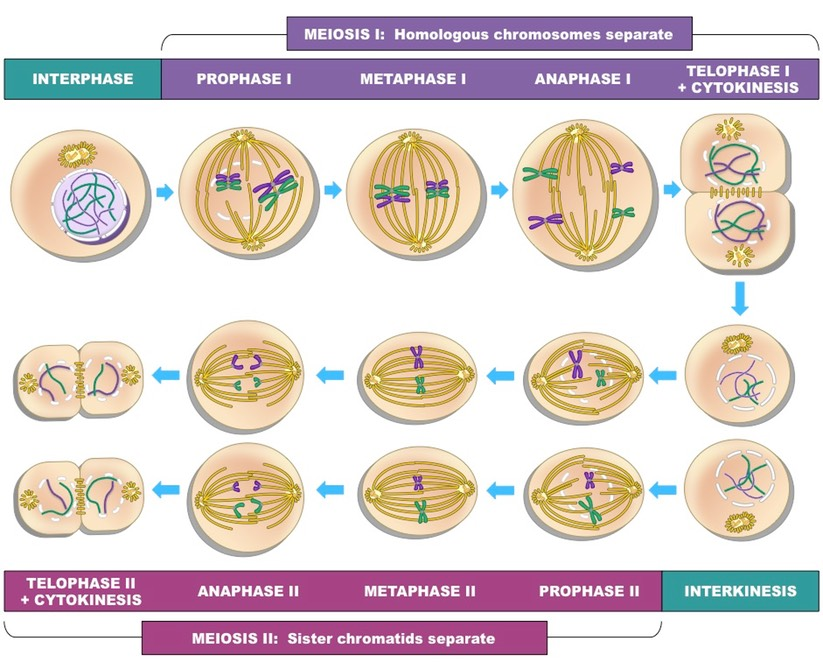
\includegraphics{./img/meiosis-complex_med.jpeg} \\
\midrule\noalign{}
\endhead
\bottomrule\noalign{}
\endlastfoot
\emph{meiosis illustration 3} \\
\end{longtable}

\begin{enumerate}
\def\labelenumi{\arabic{enumi}.}
\tightlist
\item
  interphase\\
\item
  Homologous chromosomes\\
\item
  breaks\\
\item
  middle\\
\item
  Spindle\\
\item
  homologous\\
\item
  Sister chromatids\\
\item
  two\\
\item
  Sister chromatids\\
\item
  Chromosomes; Nuclear membrane\\
\item
  align\\
\item
  pulled apart; opposite ends of the cells\\
\item
  chromosomes\\
\item
  four\\
\item
  half
\end{enumerate}

\hypertarget{homework-2}{%
\subsection{Homework}\label{homework-2}}

\textbf{Multiple Choice Questions}\\
1. A\\
2. C\\
3. D\\
4. D

\textbf{Short Answer Questions}\\
(6 points maximum) One point for each of the following:

\begin{itemize}
\tightlist
\item
  Correct description of meiosis (simply rephrasing the question earns no point)\\
\item
  DNA replicates in interphase\\
\item
  Homologous chromosomes pair in prophase I\\
\item
  Spindles move chromosomes pairs to poles in anaphase I\\
\item
  Two cycles/rounds of division in meiosis\\
\item
  No additional replication before meiosis II\\
\item
  Sister chromatids separate to poles in anaphase II\\
\item
  1 germ cell yields 4 gametes
\end{itemize}

\textbf{Fill in the Blanks}\\
1. Anaphase II\\
2. N/A\\
3. Metaphase I\\
4. Telophase II (not quite obvious)\\
5. Telophase I (not quite obvious)\\
6. N/A\\
7. Metaphase II\\
8. Prophase I\\
9. Prophase II\\
10. Anaphase I

\hypertarget{lecture-7-meiosis-3}{%
\section{Lecture 7: Meiosis-3}\label{lecture-7-meiosis-3}}

\hypertarget{lesson-outline-3}{%
\subsection{Lesson outline}\label{lesson-outline-3}}

\textbf{F. How do mitosis and meiosis differ?}\\
1. During {mitosis} and cell division, a body cell and its nucleus divide once and produce two identical cells.\\
2. During {meiosis}, a reproductive cell and its nucleus divide twice and produce four cells----two pairs of identical haploid cells.

\textbf{G. Advantages of Sexual Reproduction}\\
1. Sexual reproduction produces {offspring} that have a new combination of DNA. This results in genetic {variation} among individuals.\\
2. Genetic variation gives individuals within a population slight differences that might be an advantage if the {environment} changes.\\
3. {Selective breeding} has been used to develop desirable traits in plants and animals.

\textbf{H. Disadvantages of Sexual Reproduction}\\
1. One disadvantage of sexual reproduction is that organisms have to grow and develop until they are mature enough to produce {sex} cells.\\
2. Another disadvantage is that searching for a mate takes time and energy and might expose individuals to predators, {diseases}, or harsh environmental conditions.

Compare and contrast meiosis and mitosis and cell division
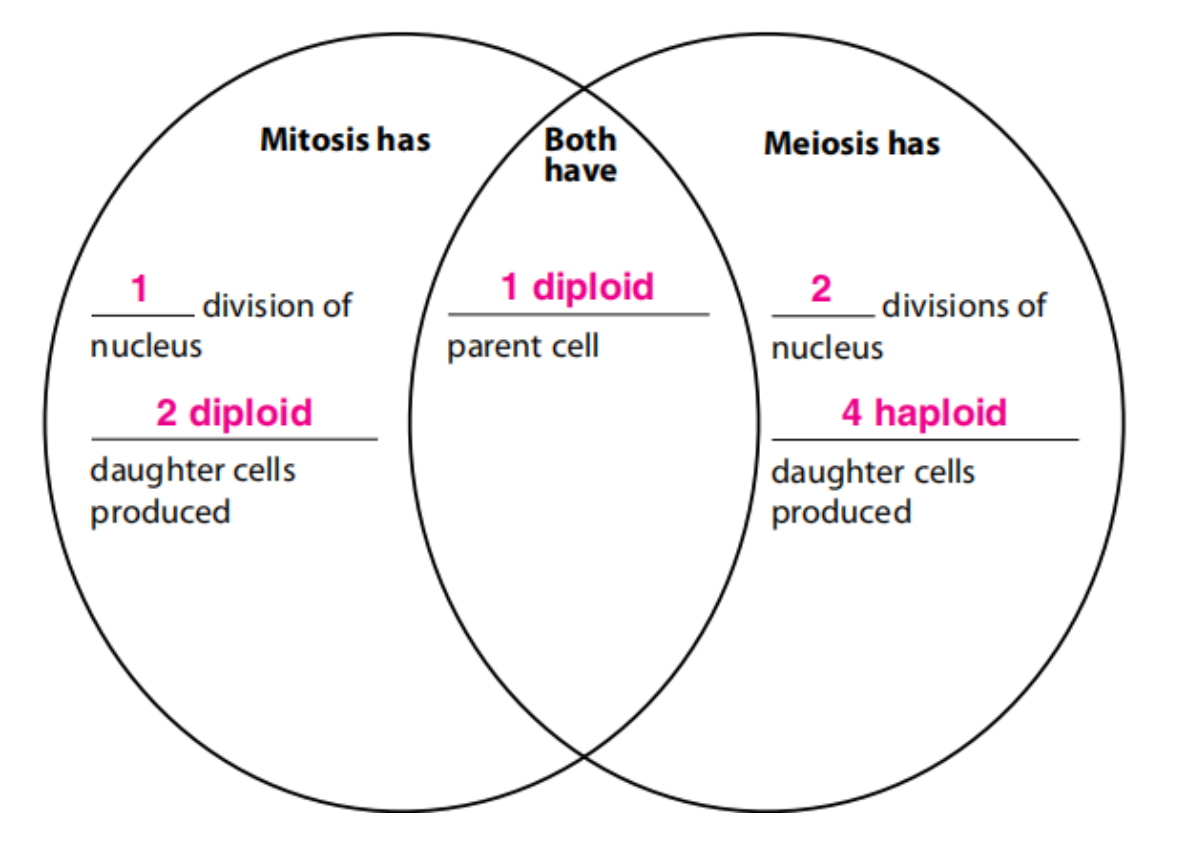
\includegraphics{./img/mitosis-meiosis.png}

\textbf{Explain} why genetic variation and selective breeding are advantages of sexual reproduction.\\
\textbf{Genetic variation}: Instead of being exact genetic copies of parents, members of the same species have different traits, which enable some of them to survive environmental changes.\\
\textbf{Selective breeding}: The process of choosing and breeding individuals with desirable traits allows breeders to create offspring with those traits.

\textbf{Identify} two main disadvantages of sexual reproduction.\\
1. takes time and takes energy\\
2. sexual reproduction is limited by certain factors (For example, fertilization cannot take place during pregnancy, which can last as long as two years in some mammals.)

\textbf{Explain} how the process of meiosis relates to the way in which a child resembles but is not an exact copy of his or her parents.\\
Observable characteristics in a child, such as \textbf{eye color, hair type and color, the shapes of facial features, and height}, resemble those of his or her parents, because the child \textbf{inherits portions of DNA from each parent}. A child is not a exact copy of his or her parents because the child \textbf{does not carry identical DNA to either parent}.

\hypertarget{lecture-8-asexual-reproduction}{%
\section{Lecture 8: Asexual Reproduction}\label{lecture-8-asexual-reproduction}}

  \bibliography{book.bib,packages.bib}

\end{document}
